\documentclass[a4paper,12pt]{extarticle}

\usepackage[utf8x]{inputenc}
\usepackage[T1,T2A]{fontenc}
\usepackage[russian]{babel}
\usepackage{hyperref}
\usepackage{indentfirst}
\usepackage{here}
\usepackage{array}
\usepackage{graphicx}
\usepackage{caption}
\usepackage{subcaption}
\usepackage{chngcntr}
\usepackage{amsmath}
\usepackage{amssymb}
\usepackage{pgfplots}
\usepackage{pgfplotstable}
\usepackage[left=2cm,right=2cm,top=2cm,bottom=2cm,bindingoffset=0cm]{geometry}
\usepackage{multicol}

\renewcommand{\le}{\ensuremath{\leqslant}}
\renewcommand{\leq}{\ensuremath{\leqslant}}
\renewcommand{\ge}{\ensuremath{\geqslant}}
\renewcommand{\geq}{\ensuremath{\geqslant}}
\renewcommand{\epsilon}{\ensuremath{\varepsilon}}
\renewcommand{\phi}{\ensuremath{\varphi}}

\counterwithin{figure}{section}
\counterwithin{equation}{section}
\counterwithin{table}{section}
\newcommand{\sign}[1][5cm]{\makebox[#1]{\hrulefill}} % Поля подписи и даты
\graphicspath{{pics/}} % Путь до папки с картинками
\captionsetup{justification=centering,margin=1cm}
\def\arraystretch{1.3}

\usepackage{courier}

\usepackage{listings}
\lstset{ %
extendedchars=\true,
keepspaces=true,
language=matlab,						% choose the language of the code
basicstyle=\scriptsize\ttfamily,		% the size of the fonts that are used for the code
numbers=left,					% where to put the line-numbers
numberstyle=\scriptsize,		% the size of the fonts that are used for the line-numbers
stepnumber=1,					% the step between two line-numbers. If it is 1 each line will be numbered
numbersep=5pt,					% how far the line-numbers are from the code
backgroundcolor=\color{white},	% choose the background color. You must add \usepackage{color}
showspaces=false				% show spaces adding particular underscores
showstringspaces=false,			% underline spaces within strings
showtabs=false,					% show tabs within strings adding particular underscores
frame=single,           		% adds a frame around the code
tabsize=2,						% sets default tabsize to 2 spaces
captionpos=b,					% sets the caption-position to bottom
breaklines=true,				% sets automatic line breaking
breakatwhitespace=false,		% sets if automatic breaks should only happen at whitespace
escapeinside={\%*}{*)},			% if you want to add a comment within your code
postbreak=\raisebox{0ex}[0ex][0ex]{\ensuremath{\color{red}\hookrightarrow\space}},
texcl=true,
inputpath=code,
showstringspaces=false,
breaklines=true
}

\begin{document}

\begin{titlepage}
\begin{center}
	\textbf{Санкт-Петербургский Политехнический Университет \\Петра Великого}\\[0.3cm]
	\small Институт компьютерных наук и технологий \\[0.3cm]
	\small Кафедра компьютерных систем и программных технологий\\[4cm]
	
	\textbf{ОТЧЕТ}\\ \textbf{по расчетному заданию}\\[0.5cm]
	\textbf{<<Идентификация сообщений, передаваемых по зашумленному каналу связи.>>}\\[0.1cm]
	\textbf{Теория вероятностей и математическая статистика}\\[8.0cm]
\end{center}

\begin{flushright}
	\begin{minipage}{0.48\textwidth}
		\begin{flushleft}
			\small \textbf{Работу выполнил студент}\\[3mm]
			\small группа 23501/4 \hspace*{6mm} Дьячков В.В.\\[5mm]
			
			\small \textbf{Преподаватель}\\[5mm]
		 	\small \sign[3cm] \hspace*{5mm} к.т.н., доц. Никитин К.В.\\[0.5cm]
		\end{flushleft}
	\end{minipage}
\end{flushright}

\vfill

\begin{center}
	\small Санкт-Петербург\\
	\small \the\year
\end{center}
\end{titlepage}

\section{Техническое задание}

По каналу связи передаются буквы $[x_1; x_2;...; x_n]$ в двоичном коде. Последовательность переданных букв образует сообщение. Канал симметричный, вероятность искажения каждого отдельного символа (бита) равна q. В результате однократной передачи сообщения $X = [x^{(1)}, x^{(2)}, ..., x^{(k)}]$ на приемной стороне принято сообщение $Y = [y_1^{(1)}, y_1^{(2)}, ..., y_1^{(k)}]$. В результате повторной передачи того же слова на приемной стороне принято слово $Y = [y_2^{(1)}, y_2^{(2)}, ..., y_2^{(k)}]$ . В результате последней ($m$-й) передачи того же слова на приемной стороне принято слово $Y = [y_m^{(1)}, y_m^{(2)}, ..., y_m^{(k)}]$.

\section{Исходные данные}

\begin{itemize}
\item Число букв: $n = 222$
\item Разрядность кода: 7 бит
\item Шум: $q = 0.168$
\item Число посылок: $m = 18$
\end{itemize}

\section{Используемые формулы}

Формула Байеса для расчета апостерирорных вероятностей:
\begin{equation}\label{eq:pxy}
	p(x_i/y_j) = \frac{p(y_j)\cdot p(x_i)}{p(y_j)}
\end{equation}

Условная вероятность приема $y_j$ при условии, что было послано $x_i$:
\begin{equation}\label{eq:pyx}
	p(y_j/x_i) = p^{k-t}\cdot q^t,
\end{equation}
где $k$ - общее количество разрядов, $t$ - количество разрядов, в которых произошла ошибка. 

Вероятность приема $y_j$:
\begin{equation}\label{eq:py}
	p(y_j) = \sum_k p(y_j/x_k)\cdot p(x_k)
\end{equation}

Энтропия ансамбля $x_i \in X$ при получении сообщения $y_j \in Y$:
\begin{equation}\label{eq:hxyj}
	H(X/y_j) = - \sum_{i=1}^n p(x_i/y_j)\cdot \log_2 p(x_i/y_j)
\end{equation}

Cовместная энтропия двух ансамблей $X$ и $Y$: 
\begin{equation}\label{eq:hxy}
	H(X/Y) = - \sum_{j=1}^n p(y_j)\cdot H(X/y_j)
\end{equation}

Среднее количество информации об $X$, полученное в сообщении $y_j$:
\begin{equation}\label{eq:ixyj}
	I(X:y_j) = - \sum_{i=1}^n p(x_i/y_j)\cdot \log_2 p(x_i) - H(X/y_j)
\end{equation}

Средняя взаимная информация, содержащаяся в $Y$ об $X$ или в $X$ об $Y$: 
\begin{equation}\label{eq:ixy}
	I(X:Y) = - H(X) - H(X/Y)
\end{equation}

\section{Последовательная передача одинаковых сообщений}

\subsection{Определение переданного сообщения}

\subsubsection{Все символы равновероятны}\label{sec:uniform}

Априорное распределение вероятностей исходных букв алфавита было задано равновероятным:
\begin{equation}
	p(x) = \frac{1}{n} = \frac{1}{222} \approx 0.0115
\end{equation}

Для вычисления апостерирорной вероятности после каждого сообщения для каждой буквы сообщения использовались формулы \ref{eq:pxy}, \ref{eq:pyx} и \ref{eq:py}.

Были построены графики изменения апостериорного распределения вероятностей на примере 7-ой буквы сообщения после каждой из 18 посылок (см. приложение 1).

По максимуму апостериорной вероятности были определены наиболее вероятные буквы и составлены варианты исходного переданного сообщения для каждой посылки:

\vspace{0.5cm}

{ \scriptsize
1: 8:ЛДь9чимв 4зЕирТПизьдпПзо:\_235\_1е Т воаНН\_пк вкаНпыпЯлдчт\_заяит пЯ геНоиб(вевЯчтаосиие\_уЗНититиса СирелЬаМр3ч1ТзаЬо,тча. Ял!Л:тогЯ(ЯоПсебмеЯТ! проСииат6(хУикРммвкеи0Ко ззЬа:и(и?ннелЯр.!А№Ч(рЯсяерн7х када-\_2!кА(и3елаА 9дЗ.

2: А,ЛА6э3инв ВаЕХр:\_изЛдОоозЕ\_235А5\_ :ЛвоШНо\_но виоНаАпАлл№т за!ет!по№теооии вето№тноТЕеЖИуЛНетиоиса (иреллаЛТ3:еТИаво,очаВ Ал:Л:тоДо(ооореиоеоТ: проре4ат!(-текОоовтеи.ио(зова:и(иеОоелЯт!!А-еЛрЯТяетнИх еадаееА.та(и3елаю(,тП,

3: !, Дь,чЛмв 4ауим, изшгттпз:\_23Ь85Зь, вЧаможно вкорпьпЯлучт еачет по№георииьверЯятнойтеЖМуЛЗеЫитиса (имикла рЕяЦсзавовича. Азя ,тоДо потрертегс: пробе4ать)хти птмвтеифие зРдпчи к(суелЯть!2-ШЛрЯсчетн7х оадания. Я(саелаю ,дП.

4: гЕ Д!ячЛов Вауим, ил(Ыттпз:\_23585\_!, вЧамжжно влоро полу№т(зачет по теории(вероятностеК уЛПекЩтина Кирилла ряяХсИавовича, АляЛ,тоДо потреитетс: проте4ат6(хти птостейшие задачи и сселАть!2-3ЛраТчетн7х завания. а саелаю(.тПВ

5: г, ДьячЛов 4ауим, из гттпз: 23Ь81\_6, воаможно вкоро получу зачет по теорииьЮероятнойтеК у Пикитина )имилйа ряяеславовица. Для ,того потребуетсю прогешать хти простеишие задачи и(сделЯть 2-3 расчетных задания. Я(саелаю ,гП!

6: Я, ДьячЛов Вауим,\_из гттпз:\_23581\_6, воаножно слоро!полу№у зачет по теории(ЮероятнойтеК у Никитина Кирелла ряяеславовичаВ Для\_этого потребуетсю проиешать эти птостейшие задачи и сделать 2-3 расчетных задания. а саелаю этП!

7: Я, Дьячков Вадим,\_из групзы 23581\_4, воаможно скоро полу№у зачет по теории Юероятнойтей у Никитина Кирилла Вячеславовица. Для\_этого потребуетсю пробешать эти прПстейшие задачи и сделЯть 2-3 расчетных задания. а саелаю эгП!

8: Я, Дьячтов Вадим,\_из групз: А3581\_4, возмжжно слоро полу№у зачет по теории вероятностей у Никитина Кирелла Вяяеславовица. Аля\_этого аотребуеося прорешать эти простейшие задачи и сделать 2-3 расчетных задания. а саелаю это!

9: Я, Дьячтов Вадим, из групз: 23581\_4, возможно скоро получу зачет по теории верЯятностей у Никитина Кирилла бячеславовица. Для этого потребуеося прорешать эти прПстейшие задачи и сделать 2-3 расчетных задания. Я саелаю это!

10: Я, Дьячтов Вадим, из групп: А3501\_4, возможно скоро полу№у зачет по теории вероятностей у Никитина Кирилла Вяяеславовича. Аля этого потребуеося прорешать эти простейшие задачи и сделать!2-3 расчетных задания. Я саелаю это!

11: Я, Дьячтов Вадим, из групп: 23501\_4, возможно скорЯ получу зачет по теории вероятностей у Никитина Кирилла Вячеславовича. Аля этого потребуется прорешать эти простейшие задачи и сделать 2-3 расчетных задания. Я сделаю это!

12: Я, Дьячтов Вадим, из групп: 23501\_4, возможно скоро получу зачет по теории вероятностей у Никитина Кирилла Вячеславовича. Аля этого потребуется прорешать эти простейшие задачи и сделать 2-3 расчетных задания. Я саелаю это!

13: Я, Дьячтов Вадим, из группы 23501\_4, возможно скоро получу зачет по теории вероятностей у Никитина Кирилла Вячеславовича. Аля этого потребуется прорешать эти простейшие задачи и сделать 2-3 расчетных задания. Я сделаю это!

14: Я, Дьячтов Вадим, из группы 23501\_4, возможно скоро получу зачет по теории вероятностей у Никитина Кирилла Вяяеславовича. Аля этого потребуется прорешать эти простейшие задачи и сделать 2-3 расчетных задания. Я сделаю это!

15: Я, Дьячтов Вадим, из группы 23501\_4, возможно скоро получу зачет по теории вероятностей у Никитина Кирилла Вячеславовича. Аля этого потребуется прорешать эти простейшие задачи и сделать 2-3 расчетных задания. Я сделаю это!

16: Я, Дьячтов Вадим, из группы 23501\_4, возможно скоро получу зачет по теории вероятностей у Никитина Кирилла Вяяеславовича. Аля этого потребуется прорешать эти простейшие задачи и сделать 2-3 расчетных задания. Я сделаю это!

17: Я, Дьячтов Вадим, из группы 23501\_4, возможно скоро получу зачет по теории вероятностей у Никитина Кирилла Вячеславовича. Для этого потребуется прорешать эти простейшие задачи и сделать 2-3 расчетных задания. Я сделаю это!

18: Я, Дьячтов Вадим, из группы 23501\_4, возможно скоро получу зачет по теории вероятностей у Никитина Кирилла Вячеславовича. Для этого потребуется прорешать эти простейшие задачи и сделать 2-3 расчетных задания. Я сделаю это!

}
\vspace{0.5cm}

Из полученных результатов видно, что только после 10 посылки исходное сообщение было распознано достаточно хорошо.

\subsubsection{Вероятности букв задаются исходя из частоты встречания}\label{sec:weghted}

В данном случае априорное распределение вероятностей исходных букв алфавита было задано исходя из частоты встречания в русском языке. Начальное распределение вероятностей стало выглядеть следующим образом:

{ \scriptsize
\begin{multicols}{6}
\noindent p('0') = 0.0115,	p('1') = 0.0115,	p('2') = 0.0115,	p('3') = 0.0115,	p('4') = 0.0115,	p('5') = 0.0115,	p('6') = 0.0115,	p('7') = 0.0115,	p('8') = 0.0115,	p('9') = 0.0115,	p('А') = 0.0328,	p('Б') = 0.0057,	p('В') = 0.0159,	p('Г') = 0.0053,	p('Д') = 0.0097,	p('Е') = 0.0307,	p('Ё') = 0.0005,	p('Ж') = 0.0030,	p('З') = 0.0069,	p('И') = 0.0283,	p('Й') = 0.0050,	p('К') = 0.0132,	p('Л') = 0.0164,	p('М') = 0.0125,	p('Н') = 0.0241,	p('О') = 0.0352,	p('П') = 0.0127,	p('Р') = 0.0210,	p('С') = 0.0207,	p('Т') = 0.0239,	p('У') = 0.0110,	p('Ф') = 0.0015,	p('Х') = 0.0035,	p('Ц') = 0.0020,	p('Ч') = 0.0048,	p('Ш') = 0.0029,	p('Щ') = 0.0019,	p('Ь') = 0.0072,	p('Ы') = 0.0080,	p('Ъ') = 0.0002,	p('Э') = 0.0006,	p('Ю') = 0.0039,	p('Я') = 0.0084,	p('а') = 0.0328,	p('б') = 0.0057,	p('в') = 0.0159,	p('г') = 0.0053,	p('д') = 0.0097,	p('е') = 0.0307,	p('ё') = 0.0005,	p('ж') = 0.0030,	p('з') = 0.0069,	p('и') = 0.0283,	p('й') = 0.0050,	p('к') = 0.0132,	p('л') = 0.0164,	p('м') = 0.0125,	p('н') = 0.0241,	p('о') = 0.0352,	p('п') = 0.0127,	p('р') = 0.0210,	p('с') = 0.0207,	p('т') = 0.0239,	p('у') = 0.0110,	p('ф') = 0.0015,	p('х') = 0.0035,	p('ц') = 0.0020,	p('ч') = 0.0048,	p('ш') = 0.0029,	p('щ') = 0.0019,	p('ь') = 0.0072,	p('ы') = 0.0080,	p('ъ') = 0.0002,	p('э') = 0.0006,	p('ю') = 0.0039,	p('я') = 0.0084,	p('.') = 0.0115,	p(',') = 0.0115,	p('!') = 0.0115,	p(':') = 0.0115,	p('?') = 0.0115,	p('-') = 0.0115,	p('\_') = 0.0115,	p('№') = 0.0115,	p('(') = 0.0115,	p(')')\ \ \ =\ \ \ \ 0.0115,\\	p('\ ')\ \ \ =\ \ \ \ 0.0115.
\end{multicols}

}

Аналогичным образом были построены графики изменения апостериорного распределения вероятностей на примере 7-ой буквы сообщения после каждой из 18 посылок (см. приложение 2).

По максимуму апостериорной вероятности были определены наиболее вероятные буквы и составлены варианты исходного переданного сообщения для каждой посылки:

\vspace{0.5cm}
{ \scriptsize
1: 8:ЛДь,чимв 4зЕирТПизьдпПзо:\_235\_1е Т воаНН\_пк вкаНпыпЯлдчт\_заяит пЯ геНоиб(вевЯчтаосиие\_уЗНититиса СирелЬаМр3ч1ТзаЬо,тча. Ял!Л:тогЯ(ЯоПсебмеЯТ! проСииат6(хУикРммвкеи0Ко ззЬа:и(и?ннелЯр. А№Ч(рЯсяерн7х када-\_2!кА(и3елаА ,дЗ.

2: А:ЛА6э3инв ВаЕХр:\_изЛдОоозЕ\_275А9? :ЛвоШНо\_но виоНаАпАлл№т за:ет по№теооии вето№тноТЕеЖИуЛНетиоиса )иреллаЛТ3:еТИаво,очаВ Ал:Л:тоДо ооореиоеоТ: проре4ат!)-текОоовтеи.ио зова:и иеОоелЯт! А-еЛрЯТяетнИх еадаееА.та)и3елаю ,тП,

3: !, Дь,чЛмв 4ауим, изшгттпз:\_23Ь85Зь, вЧаможно вкорпьпЯлучт еачет по№георииьверЯятнойтеЖМуЛЗеЫитиса (имикла рЕяЦсзавовича. Азя ,тоДо потрертегс: пробе4ать)хти птмвтеифие зРдпчи к(суелЯть 2-ШЛрЯсчетн7х оадания. Я(саелаю ,дП.

4: гЕ Д!ячЛов Вауим: ил Ыттпз:\_23585\_6, вЧамжжно влоро полу№т зачет по теории вероятностеК уЛПекЩтина Кирилла ряяХсИавовича. АляЛ,тоДо потреитетс: проте4ат6)хти птостейшие задачи и сселАть 2-3ЛраТчетн7х завания. а саелаю ,тПВ

5: г, ДьячЛов 4ауим, из гттпз: 23Ь81\_6, воаможно вкоро получу зачет по теорииьЮероятнойтеК у Пикитина )имилйа ряяеславовица. Для ,того потребуетсю прогешать хти простеишие задачи и(сделЯть 2-3 расчетных задания. Я(саелаю ,гП!

6: Я, ДьячЛов Вауим,\_из гттпз:\_23581\_6, воаножно слоро полу№у зачет по теории ЮероятнойтеК у Никитина Кирелла ряяеславовичаВ Для\_этого потребуетсю проиешать эти птостейшие задачи и сделать 2-3 расчетных задания. а саелаю этП!

7: Я, Дьячков Вадим,\_из групзы 23581\_4, воаможно скоро полу№у зачет по теории Юероятнойтей у Никитина Кирилла Вячеславовица. Для\_этого потребуетсю пробешать эти прПстейшие задачи и сделЯть 2-3 расчетных задания. а саелаю эгП!

8: Я, Дьячтов Вадим,\_из групз: А3581\_4, возмжжно слоро полу№у зачет по теории вероятностей у Никитина Кирелла Вяяеславовица. Аля этого аотребуеося прорешать эти простейшие задачи и сделать 2-3 расчетных задания. а саелаю это!

9: Я, Дьячтов Вадим, из групз: 23581\_4, возможно скоро получу зачет по теории верЯятностей у Никитина Кирилла бячеславовица. Для этого потребуеося прорешать эти прПстейшие задачи и сделать 2-3 расчетных задания. Я саелаю это!

10: Я, Дьячтов Вадим, из групп: А3501\_4, возможно скоро полу№у зачет по теории вероятностей у Никитина Кирилла Вяяеславовича. Аля этого потребуеося прорешать эти простейшие задачи и сделать 2-3 расчетных задания. Я саелаю это!

11: Я, Дьячтов Вадим, из групп: 23501\_4, возможно скорЯ получу зачет по теории вероятностей у Никитина Кирилла Вячеславовича. Аля этого потребуется прорешать эти простейшие задачи и сделать 2-3 расчетных задания. Я сделаю это!

12: Я, Дьячтов Вадим, из групп: 23501\_4, возможно скоро получу зачет по теории вероятностей у Никитина Кирилла Вячеславовича. Аля этого потребуется прорешать эти простейшие задачи и сделать 2-3 расчетных задания. Я саелаю это!

13: Я, Дьячтов Вадим, из группы 23501\_4, возможно скоро получу зачет по теории вероятностей у Никитина Кирилла Вячеславовича. Аля этого потребуется прорешать эти простейшие задачи и сделать 2-3 расчетных задания. Я сделаю это!

14: Я, Дьячтов Вадим, из группы 23501\_4, возможно скоро получу зачет по теории вероятностей у Никитина Кирилла Вяяеславовича. Аля этого потребуется прорешать эти простейшие задачи и сделать 2-3 расчетных задания. Я сделаю это!

15: Я, Дьячтов Вадим, из группы 23501\_4, возможно скоро получу зачет по теории вероятностей у Никитина Кирилла Вячеславовича. Аля этого потребуется прорешать эти простейшие задачи и сделать 2-3 расчетных задания. Я сделаю это!

16: Я, Дьячтов Вадим, из группы 23501\_4, возможно скоро получу зачет по теории вероятностей у Никитина Кирилла Вяяеславовича. Аля этого потребуется прорешать эти простейшие задачи и сделать 2-3 расчетных задания. Я сделаю это!

17: Я, Дьячтов Вадим, из группы 23501\_4, возможно скоро получу зачет по теории вероятностей у Никитина Кирилла Вячеславовича. Для этого потребуется прорешать эти простейшие задачи и сделать 2-3 расчетных задания. Я сделаю это!

18: Я, Дьячтов Вадим, из группы 23501\_4, возможно скоро получу зачет по теории вероятностей у Никитина Кирилла Вячеславовича. Для этого потребуется прорешать эти простейшие задачи и сделать 2-3 расчетных задания. Я сделаю это!

}
\vspace{0.5cm}

Из результатов видно, что в ситуации, когда вероятности задаются ихсодя из частоты встречания букв в русском языке, зашумленное сообщение было распознано немного быстрее, причем существенное отличие наблюдается только после нескольких первых посылок.

\subsection{Расчет энтропии и количества информации}

Выберем в посылаемом сообщении произвольную букву под номером 7, далее все вычисления будут относиться к этой букве.

Для вычисления апостерирорной вероятности после каждого сообщения для каждой буквы сообщения использовались формулы \ref{eq:pxy}, \ref{eq:pyx} и \ref{eq:py}.

По формулам \ref{eq:hxyj} и \ref{eq:hxy} были вычислены условные энтропии на сообщения $j_y$ и средняя условная энтропия $H(X/y)$ соответственно. 

\begin{multicols}{2}
\begin{center}
Равновероятные:\\
$H(X|Y) = 0.86169$\\
Взвешенные вероятности:\\
$H(X|Y) = 1.23544$
\end{center}
\end{multicols}

На рисунке \ref{plt:entropy} изобрежен график изменения условной энтропии $H(X/y_j)$ от номера посылки.

\begin{figure}[H]
\begin{center}
	\vspace{-0.5cm}
	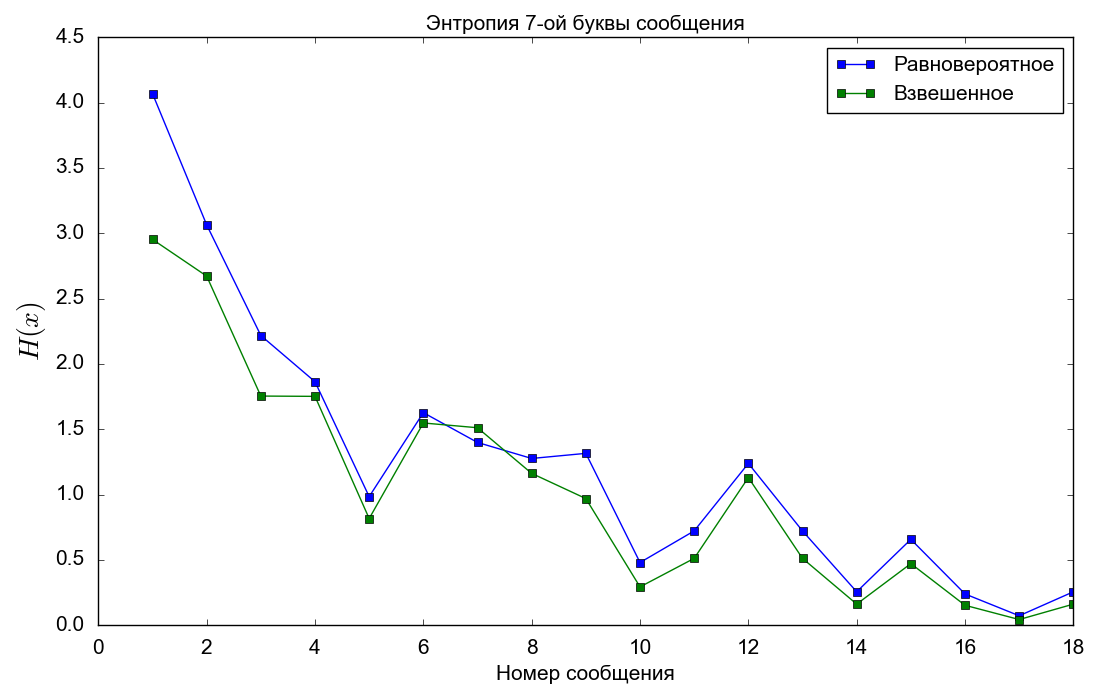
\includegraphics[scale=0.62]{entropy}
	\caption{}
	\label{plt:entropy}
	\vspace{-0.5cm}
\end{center}
\end{figure}

По формулам \ref{eq:ixyj} и \ref{eq:ixy} были определены среднее количество информации $I(X, y_j)$ об $X$, содержащееся в $y_j$ и средняя взаимная информация $I(X, Y)$.

\begin{multicols}{2}
\begin{center}
Равновероятные:\\
$I(X|Y) = 5.58125$\\
Взвешенные вероятности:\\
$I(X|Y) = 4.79441$
\end{center}
\end{multicols}

На рисунке \ref{plt:info} изобрежен график изменения количества
информации $I(X, y_j)$ от номера посылки.

\begin{figure}[H]
\begin{center}
	\vspace{-0.5cm}
	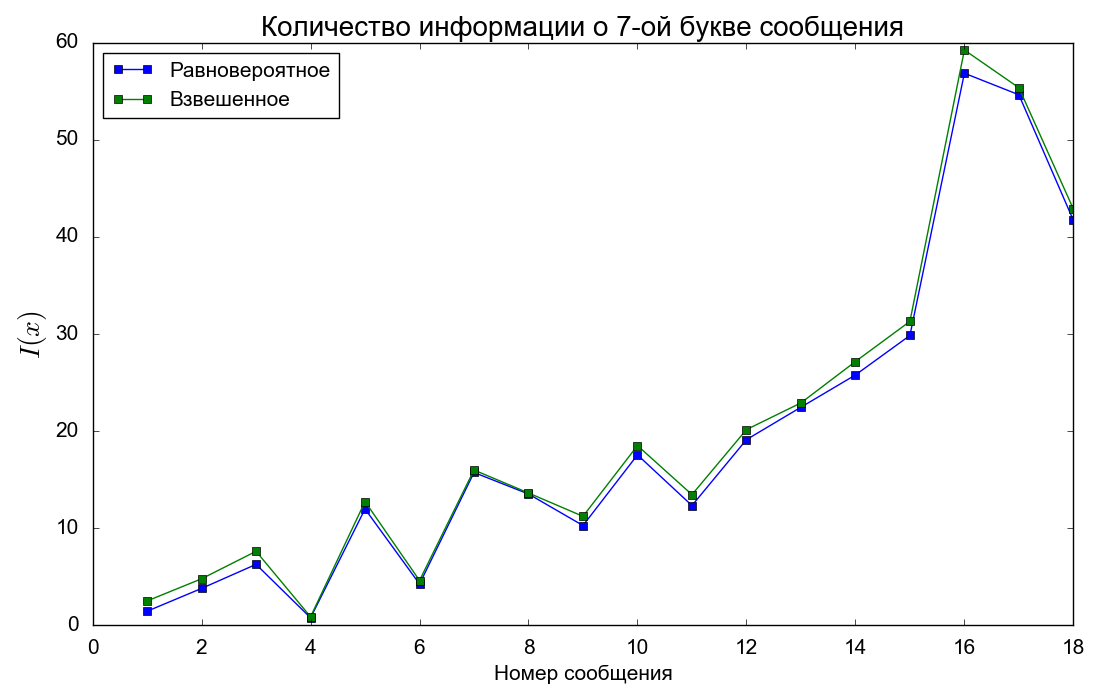
\includegraphics[scale=0.62]{infos}
	\caption{}
	\label{plt:info}
	\vspace{-0.5cm}
\end{center}
\end{figure}

\section{Передача сообщения многократным дублированием}

Рассмотрим $m$ передач сообщений как передачу одного большого сообщения, в котором каждый символ многократно ($m$-кратно) дублируется. При этом новый алфавит по сути это $m$-кратное дублирование старого алфавита.

\subsection{Определение переданного сообщения}

\subsubsection{Все символы равновероятны}

Априорное распределение вероятностей исходных букв алфавита было задано равновероятным, так же как в пункте \ref{sec:uniform}.

Для вычисления апостерирорной вероятности для каждой буквы сообщения использовались формулы \ref{eq:pxy}, \ref{eq:pyx} и \ref{eq:py}.

По максимуму апостериорной вероятности были определены наиболее вероятные буквы и составлены варианты исходного переданного сообщения для каждой посылки:

\vspace{0.5cm}
{ \scriptsize

Я, Дьячтов Вадим, из группы 23501\_4, возможно скоро получу зачет по теории вероятностей у Никитина Кирилла Вячеславовича. Для этого потребуется прорешать эти простейшие задачи и сделать 2-3 расчетных задания. Я сделаю это!

}
\vspace{0.5cm}

На рисунке \ref{plt:long_uniform} изображен график изменения апостериорного распределения вероятностей на примере 7-ой буквы сообщения.

\begin{figure}[H]
\begin{center}
	\vspace{-0.9cm}
	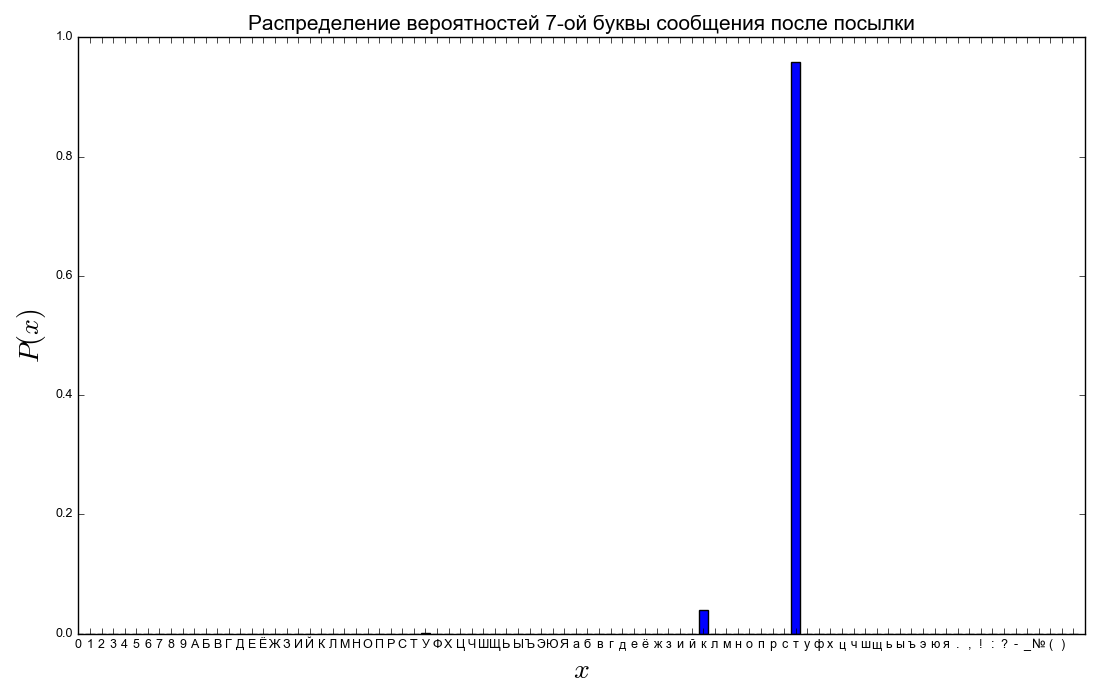
\includegraphics[scale=0.62]{long_uniform}
	\caption{}
	\label{plt:long_uniform}
	\vspace{-0.5cm}
\end{center}
\end{figure}

\subsubsection{Вероятности букв задаются исходя из частоты встречания}

В данном случае априорное распределение вероятностей исходных букв алфавита было задано исходя из частоты встречания в русском языке, как в пункте \ref{sec:weghted}.

\begin{figure}[H]
\begin{center}
	\vspace{-0.9cm}
	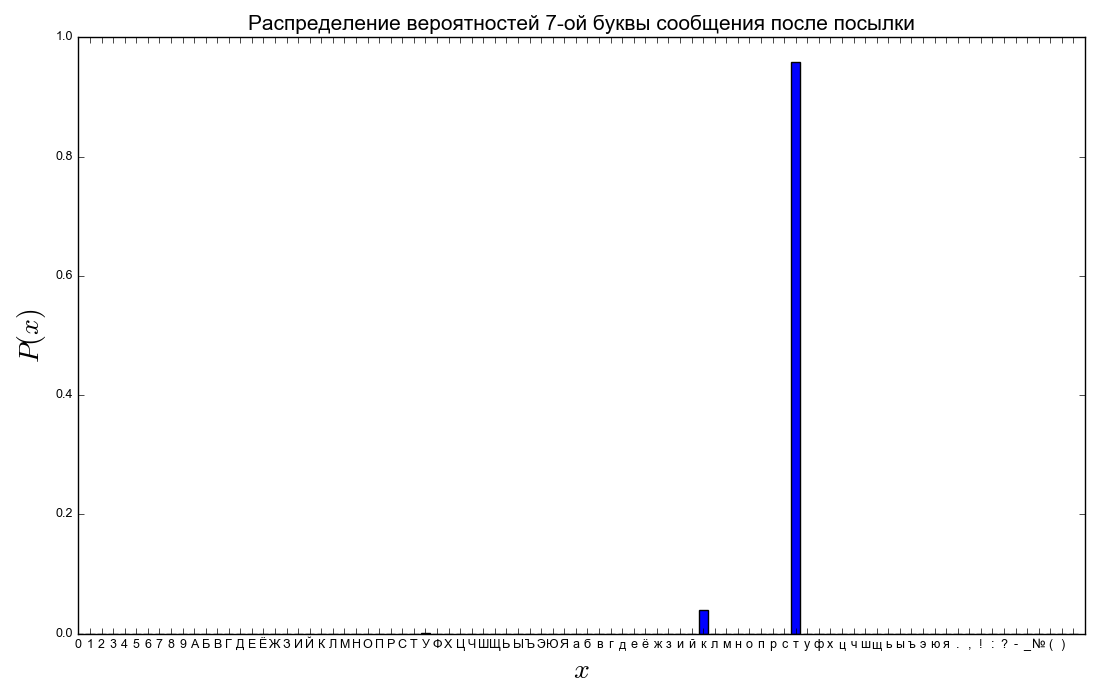
\includegraphics[scale=0.62]{long_uniform_weighted}
	\caption{}
	\label{plt:long_uniform_weighted}
	\vspace{-0.5cm}
\end{center}
\end{figure}

На рисунке \ref{plt:long_uniform_weighted} изображен график изменения апостериорного распределения вероятностей на примере 7-ой буквы сообщения при задании ариорных вероятсней исходя из частоты встречания букв в русском языке.

По максимуму апостериорной вероятности были определены наиболее вероятные буквы и составлены варианты исходного переданного сообщения для каждой посылки:

\vspace{0.5cm}
{ \scriptsize

Я, Дьячтов Вадим, из группы 23501\_4, возможно скоро получу зачет по теории вероятностей у Никитина Кирилла Вячеславовича. Для этого потребуется прорешать эти простейшие задачи и сделать 2-3 расчетных задания. Я сделаю это!

}
\vspace{0.5cm}

В обоих случаях, когда априорные вероятности распределены равновмерно и априорные вероятности были заданы в зависимости от частоты встречания в русском языке, конечные результаты оказались идентичны.

\subsection{Расчет энтропии и количества информации}

Выберем в посылаемом сообщении произвольную букву под номером 7, далее все вычисления будут относиться к этой букве.

Для вычисления апостерирорной вероятности после каждого сообщения для каждой буквы сообщения использовались формулы \ref{eq:pxy}, \ref{eq:pyx} и \ref{eq:py}.

По формулам \ref{eq:hxyj} и \ref{eq:hxy} были вычислены условные энтропии на сообщения $j_y$ и средняя условная энтропия $H(X/y)$ соответственно. 

\begin{multicols}{2}
\begin{center}
Равновероятные:\\
$H(X|y_7) = 0.25627$\\
$H(X|Y) = 0.01639$\\
Взвешенные вероятности:\\
$H(X|y_7) = 0.16181$\\
$H(X|Y) = 0.01845$
\end{center}
\end{multicols}

По формулам \ref{eq:ixyj} и \ref{eq:ixy} были вычислены среднее количество информации об $X$, полученное в сообщении $y_j$ и средняя взаимная информация, содержащаяся в $Y$ об $X$ или в $X$ об $Y$: 

\begin{multicols}{2}
\begin{center}
Равновероятные:\\
$I(X:y_7) = 6.18666$\\
$I(X:Y) = 6.42655$\\
Взвешенные вероятности:\\
$I(X:y_7) = 5.24499$\\
$I(X:Y) = 6.01141$
\end{center}
\end{multicols}

Из результатов видно, что значения энтропии и количества инфрормации при последовательной передачи одинаковых сообщений и при передаче сообщения многократным дублированием оказались близки.

\section{Выводы}

В процессе работы при помощи формулы Байеса было идентифицировано сообщение, передаваемое по зашумленному каналу связи. Передача была рассмотрена как последовательнность одинаковых сообщений и как передача сообщения многократным дублированием. При этом были рассмотрены два варианта: 
\begin{itemize}
\item все символы равновероятны;
\item вероятности букв задаются исходя из частоты встречания.
\end{itemize}
Для каждой посылки была найдена условная энтропия и количество информации, содержащееся в сообщении, а так же построены графики распределения вероятносей на примере одной из букв сообщения. Листинг программы приведен в приложении 3.

\section*{Приложение 1. Изменение распределения апостериорных вероятностей для равноверотяных символов}

\foreach \n in {1,...,18}{%
	\begin{figure}[H]
	\begin{center}
		\vspace{-0.5cm}
		\includegraphics[scale=0.62]{uniform\n}
		\vspace{-1cm}
	\end{center}
	\end{figure}
}

\section*{Приложение 2. Изменение распределения апостериорных вероятностей для взвешенных вероятностей символов}

\foreach \n in {1,...,18}{%
	\begin{figure}[H]
	\begin{center}
		\vspace{-0.5cm}
		\includegraphics[scale=0.62]{weighted\n}
		\vspace{-1cm}
	\end{center}
	\end{figure}
}

\newpage

\section*{Приложение 3. Исходный код программы}

\captionof{lstlisting}{probability.py}
\lstinputlisting[language=Python,
	basicstyle=\scriptsize,	
	numberstyle=\scriptsize]{probability.py}

\end{document}